\documentclass[11pt,a4paper,oneside]{book}
\usepackage{hyperref}
\usepackage[T1]{fontenc}
\usepackage[francais]{babel}
\usepackage[utf8]{inputenc}
\usepackage{url}
\usepackage{tikz}
\usetikzlibrary{automata}
\usepackage{amsmath}
\usepackage{amssymb}
\usepackage{marginnote}
\usepackage[left=1cm,right=4cm,marginparwidth=3cm]{geometry}
\usepackage{amsmath}
\usepackage{enumitem}
\usepackage{wrapfig}

%FIXME mettre en évidence les définitions et propriétés ?
%FIXME pour les mathématiciens, donner de quoi le faire à la main : à partir de
%la séparation, montrer le paquet et donner le résumé qu'ils utiliseront

\title{Dansez maintenant !}
\author{Guillaume \textsc{Huysmans}}%, Quentin \textsc{Carpentier}}
\begin{document}
\maketitle
%FIXME cigale et la fourmi comme couverture !!
\emph{Le problème décrit ici dérive d'Advent of Code
\footnote{\url{https://adventofcode.com/2017/day/16}},
un calendrier de l'Avent avec
des problèmes algorithmiques au lieu de chocolats.}
\marginpar{le dire !}

Une société de petits personnages adore la danse. Chaque année, pour Noël, ils
organisent une grande fête à laquelle leur Grande Reine Vénérée participe. Sa
Majesté n'autorise pas tout et n'importe quoi : seules les danses qui La font
commencer et finir à la première place sont permises.
Si elle finit à une autre place, le
chorégraphe est exécuté. C'est ce qui est arrivé au chorégraphe de la Cour
l'année passée : il faut dire qu'avec son grand âge, il n'avait déjà plus toute
sa tête. Cette année, c'est à son fils de prendre la relève : tous les autres
ont bien trop peur de mourir pour un pas de travers. Il doit faire quelque
chose de grandiose s'il veut faire oublier l'erreur de son père et profiter de
ses cadeaux sous le sapin.
Le problème, c'est qu'il a laissé tomber ses papiers quelques
jours avant Noël et qu'il avait oublié de les numéroter.
Il a presque réussi à les remettre dans l'ordre mais il hésite entre deux
possibilités et il n'a plus le temps de les essayer.

Ils commencent dans l'ordre ($A\dots P$) et enchaînent trois types de pas :
\begin{itemize}
\item \texttt{spin} $n$ ($\forall n \in \{1\dots15\}$) :
	\marginpar{expliquer la notation : $\forall x \in E$...}
	les $n$ derniers viennent devant les premiers. \\
	Par exemple, \texttt{spin 1} sur \texttt{DACB} donne \texttt{BDAC}.
\item \texttt{exchange} $i$ $j$ ($\forall i,j \in \{0\dots15\}$) :
	ceux en $i$ et $j$ échangent leur place. \\
	Par exemple, \texttt{exchange 0 2} sur \texttt{CBDA} donne \texttt{DBCA}.
\item \texttt{partner} $a b$ ($\forall a,b \in \{A\dots P\}$) :
	$a$ et $b$ échangent leur place.
	\marginpar{ne pas confondre} \\
	Par exemple, \texttt{partner A D} sur \texttt{DBAC} donne \texttt{ABDC}.
\end{itemize}

\chapter{Simulation}\label{ch:sim}
%\section{Exploration}
Pour simplifier nos exemples, nous commencerons avec seulement quatre couleurs
(pour quatre personnages).
\newcommand{\boxes}{
	$\begin{array}{|l|l|l|l|}\hline
	\phantom{a} & \phantom{a} & \phantom{a} & \phantom{a} \\ \hline
	\end{array}$
}
Par groupes, travaillez sur ces exercices :
\begin{enumerate}
\item \emph{Décrivez} l'étape nécessaire au fonctionnement de \texttt{partner}.
	\emph{Écrivez} sa déclaration.
\item \emph{Complétez} ces schémas puis \emph{implémentez} ces pas en Pascal :
	\marginpar{cases vides !!}
	\begin{enumerate}
	\item \boxes \texttt{procedure spin(n: 1..15);}
	\item \boxes \texttt{procedure exchange(i, j: 0..15);}
	\item \boxes \texttt{procedure partner(a, b: 'A'..'P');}
	\end{enumerate}
\item \emph{Simulez} les étapes successives de cette danse :
\marginpar{couleurs dans leur dos pour ne pas les voir direct'}
	\begin{enumerate}
	%FIXME indices !! surtout pas confondre avec ce qu'on fera plus loin
	\item \boxes \boxes (positions initiales)
	\item \boxes \boxes \texttt{spin 3}
	\item \boxes \boxes \texttt{partner B D}
	\item \boxes \boxes \texttt{exchange 0 1}
	\item \boxes \boxes \texttt{spin 1}
	\item \boxes \boxes \texttt{exchange 2 3} \label{sim:last}
	\end{enumerate}
\item En permutant deux pas, le résultat change...
	(\emph{entourez et justifiez} la bonne réponse) :
	\begin{enumerate}
		\item toujours ? \marginpar{$x_{01}\circ x_{23}$}
		\item jamais ? \marginpar{$x_{01}\circ x_{12}$}
		\item parfois ?
	\end{enumerate}
\item \emph{Vrai ou faux ? Expliquez. }
	<<~En partant de (\ref{sim:last}), les personnages se déplaceront encore de
	la même manière s'ils entament une deuxième fois la même danse.~>>
	\marginpar{$p_{AC}\circ x_{01}$}
\item Schématisez une manière d'aider notre chorégraphe favori.
\end{enumerate}

\chapter{Optimisations}
Grâce à vous, Noël s'est bien passé, notre ami a survécu.
Il nous doit une \emph{reconnaissance éternelle}
mais il a encore un <<~petit quelque chose~>> à nous demander.

Sa~Majesté se lasse de tout ça et a décidé de changer les règles :
pendant le prochain milliard d'années (ils vivent tous très longtemps mais la
principale cause de mortalité est la décapitation), l'Élu
(qu'Elle essaiera de ne pas exécuter entre-temps, Elle fera un effort)
participera à sa place et ils reprendront du même endroit l'année suivante.
%Grâce à ses talents de négociateur, il a pu obtenir de Sa~Majesté qu'elle
%accepte plus de danses originales (Elle n'est plus toujours première à la fin)
%à condition qu'après un milliard d'années, Elle finisse à nouveau la première.
La danse ne changera pas (quel intérêt si Elle ne regarde pas ?).
Le chorégraphe doit maintenant prédire la position exacte des danseurs après
tout ce temps. S'il se trompe, il sera exécuté, lui et toute sa famille.
%Son règne n'est pas près de s'arrêter : Sa~Majesté est immortelle.

Exercice : combien de temps nous faudrait-il pour simuler ça ?

\section{Suite}\label{sec:suite}
Si on écrit $d(x)$ le résultat de la danse $d$ sur les positions des danseurs
$x$, les positions à la fin de chaque danse peuvent être modélisées à l'aide
d'une suite :\[
	\forall n \in \mathbb{N} \quad u_n =
	\left\{\begin{array}{ll}
		\texttt{ABCDEFGHIJKLMNOP} & \text{si $n=0$} \\
		d\left(u_{n-1}\right) & \text{sinon}
	\end{array}\right.
\]

Il se peut qu'il ne soit pas nécessaire de calculer $u_{1000000000}$ : \[
	\exists i<j \in \mathbb{N} \quad
	u_i=u_j \implies
	\left(\forall n \geq j : u_n=u_{n-j+i}\right)
	%\left(\forall n \in \mathbb{N} : n\geq j \implies d_n=d_{n-(j-i)}\right)
\]

Puisque $i<j \iff \exists k \in \mathbb{N}_0 : j=i+k$, on peut éliminer les
tours inutiles (voir figure \ref{fig:cycle}) :
\marginpar{Euclide}
\[
	\exists i \in \mathbb{N}, k \in \mathbb{N}_0 \quad
	u_i=u_{i+k} \implies
	\left(\forall n \geq i : u_n=u_{i+(n-i)\text{ mod } k}\right)
\]
%FIXME?

\begin{figure}[ht]
	\centering
	\begin{tikzpicture}[node distance=1.5cm]
		\node (0) {$u_0$};
		\node (1) [right of=0] {$u_1$};
		\node (2) [right of=1] {$u_2$};
		\node (i) [right of=2] {$u_i$};
		\node (i+1) [right of=i] {$u_{i+1}$};
		\node (i+2) [right of=i+1] {$u_{i+2}$};
		\node (j) [above of=i,node distance=1cm] {$u_j$};
		\node (j+1) [above of=i+1,node distance=1cm] {$u_{j+1}$};
		\node (j+2) [above of=i+2,node distance=1cm] {$u_{j+2}$};
		\draw (0) edge[->] node [above,midway] {$d$} (1);
		\draw (1) edge[->] node [above,midway] {$d$} (2);
		\draw (2) edge[->] node [above,midway] {$\dots$} (i);
		\draw (i) edge[->] node [above,midway] {$d$} (i+1);
		\draw (i+1) edge[->] node [above,midway] {$d$} (i+2);
		\draw (i+2) edge[->,bend left] node [below,midway] {$\dots$} (i);
		%\draw (j) edge[->] node [above,midway] {$d$} (j+1);
		%\draw (j+1) edge[->] node [above,midway] {$d$} (j+2);
		%\draw (j+2) edge[->,bend right] node [above,midway] {$\dots$} (j);
		\draw (i) edge[double equal sign distance] (j);
		\draw (i+1) edge[double equal sign distance] (j+1);
		\draw (i+2) edge[double equal sign distance] (j+2);
	\end{tikzpicture}
	\caption{Suite périodique}
	\label{fig:cycle}
\end{figure}

En pratique, la période $k$ peut être assez longue, c'est pourquoi on ne
stockera pas toutes les valeurs en mémoire. La \emph{conclusion} de cette
implication nous donne une façon de calculer $u_n$ quand $n\geq i$ (on espère
que $i\ll n$...) mais nous avons besoin de calculer $k$ et $i$.

Ce problème a déjà été étudié en théorie des graphes (un graphe est un ensemble
de \emph{points} ou \emph{noeuds} reliés par \emph{arêtes})
et nous allons redécouvrir l'\emph{algorithme du lièvre et de la tortue}.

\section{Profilage}
Un \emph{profiler} permet (entre autres) de connaître la proportion de temps
passé dans une partie d'un programme en inspectant régulièrement l'état d'un
programme. Voici ce qu'il nous a appris :
\begin{itemize}
\item \texttt{partner} passe beaucoup de temps à chercher où se trouvent les
	caractères à intervertir.
\item \texttt{spin} modifie toujours chaque case du tableau.
\end{itemize}

\begin{figure}[ht]
	\centering
	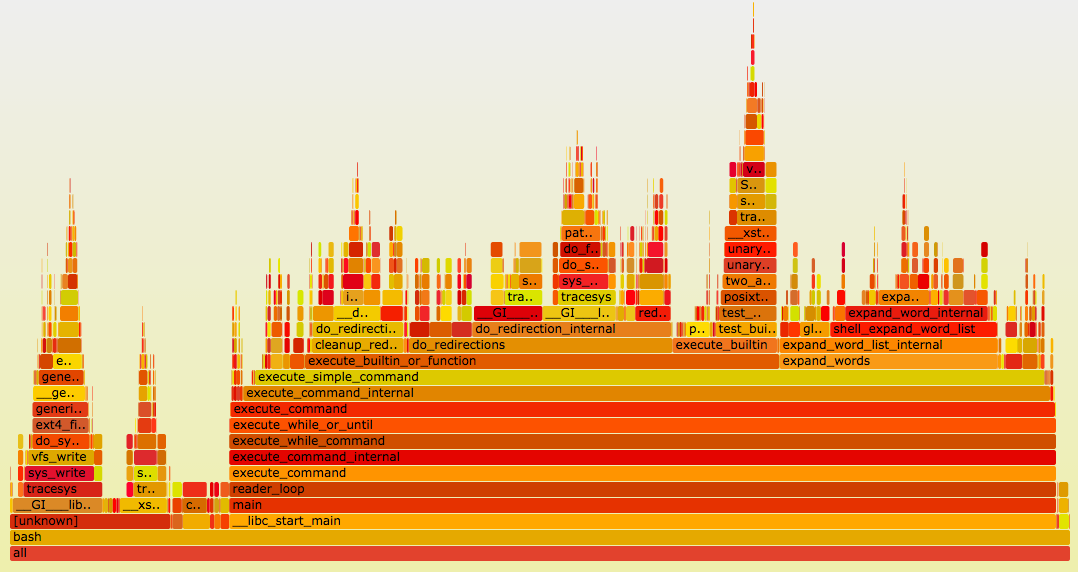
\includegraphics[width=0.7\linewidth]{cpu-bash-flamegraph.png}
	\caption{\emph{Flame graph} créé par
	\url{https://github.com/brendangregg/FlameGraph}}
	\label{fig:flamegraph}
\end{figure}

\section{Sur un cercle}
Imaginons maintenant que les danseurs se trouvent sur un cercle.

\begin{wrapfigure}[8]{r}{0.4\textwidth}
	\centering
	\begin{tikzpicture}
		\draw (0,0) circle [radius=0.7cm];
		\draw (0,0) circle [radius=1.4cm];
		\draw (0,0) circle [radius=2.1cm];
		%\foreach \angle [count=\xi] in {0,90,180,270} {
			%\draw[dashed] (\angle:0.2cm) -- (\angle:2cm);
		%}
	\end{tikzpicture}
	\caption{Cercle (à compléter !)}
	\label{fig:circle}
\end{wrapfigure}

Par groupes, répondez à ces questions :

\begin{enumerate}
\item Où se trouve le premier danseur ?
\item Y a-t-il plusieurs façons de lire un tel schéma ?
	\marginpar{sens de rotation}
\item Que fait \texttt{spin 2} ? Est-ce que ça va plus vite ?
	\marginpar{compter à partir de la flèche}
\item Que fait \texttt{exchange 0 3} après \texttt{spin 2} ?
\item Un tableau est-il encore adapté ?
	\marginpar{plier, montre.}
	\begin{itemize}
	\item Si c'est le cas, représentez-le à plat.
	\item Sinon, expliquez pourquoi c'est impossible.
	\end{itemize}
\end{enumerate}

\marginpar{optimisé \texttt{spin}, isomorphe tab}

\section{Transformations}
On peut s'occuper séparément des positions et des personnages :
\begin{itemize}
	\item \texttt{spin} et \texttt{exchange} ne dépendent pas des personnages.
	\item \texttt{partner} ne dépend pas des positions.
\end{itemize}

De cette façon, ces deux familles de pas n'<<~interfèrent~>> plus comme on le
voyait à la fin du chapitre \ref{ch:sim} et
il devient possible (et utile !) de les résumer séparément.

%FIXME comment les utiliser

\subsection{Tableaux}
Changeons totalement notre manière de voir les choses : puisqu'on peut échanger
séparément les personnages, on peut utiliser un tableau indicé
\marginpar{structure $\neq$ de celle employée par la simulation
	pour ne pas confondre}
par un personnage (\texttt{subst: array['A'..'P'] of 'A'..'P'}) afin d'associer
à chacun celui avec lequel il a été échangé.
Le tableau ne stocke plus où se trouvent les personnages mais décrit
comment les échanger.

Cette définition peut paraître étrange : habituellement, on indice un tableau
avec un entier, pas un caractère. En réalité, on peut voir un caractère
comme un entier sur un octet\footnote{Ce n'est pas vrai en général ($\pi$...)
mais nous n'utilisons que les lettres de A à P. Un~octet (\emph{byte}) est
composé de 8~bits (0 ou 1), ce qui fait seulement $2^8=256$ possibilités, donc
pas assez pour ne serait-ce que le chinois.} : en ASCII,
les majuscules commencent à 65 et se suivent, donc B=66, C=67, etc. Il peut
alors retirer 65 de chaque lettre pour obtenir des indices dans $\{0..15\}$ :

\begin{table}[h]
\center
\begin{tabular}{c|c|c}
Lettre & ASCII & Indice \\ \hline\hline
A & 65 & 0 \\ \hline
B & 66 & 1 \\ \hline
C & 67 & 2 \\ \hline
\dots & \dots & \dots \\ \hline
P & 80 & 15
\end{tabular}
\caption{Équivalence d'indices}
\end{table}

Par groupes, travaillez sur ces exercices :
\begin{enumerate}
\item \boxes Que contient le tableau avant le premier \texttt{partner x y} ?
	\marginpar{indices !}
\item \boxes Construisez un tableau qui ne représente que \texttt{partner A B}.
	\marginpar{dessiner les rails équivalents}
\item \boxes Construisez un autre tableau représentant \texttt{partner B C}.
\item \boxes Comment pourriez-vous les résumer (\emph{composer}) ?
	L'ordre importe-t-il ?
	\marginpar{rails connectés}
\item \boxes Comment appliquer le dernier tableau à la
		situation initiale \texttt{BDCA} ? \\
	\boxes Notez ici le résultat de la simulation et comparez.
\item \boxes Comment faire un tableau qui a pour effet d'\emph{inverser} celui
	d'un autre ?
\end{enumerate}

%TODO schéma pages résumées

\subsection{Fonctions}
Mathématiquement, un tableau présenté ci-dessus peut aussi être vu comme une
\emph{fonction} qui prend comme paramètre un personnage, et qui change au fur et
à mesure qu'on <<~apprend~>> les pas de la danse.
Puisqu'il y a un nombre fini de personnages, on peut leur attribuer une case à
chacun. On est aussi capable de comparer deux fonctions : cela revient à
comparer les tableaux qui les décrivent.

\subsubsection{Algèbre}
Pourquoi raisonner de manière abstraite ?
\marginpar{métaphore entrée Disneyland}
\begin{itemize}
\item pour s'éloigner d'exemples particuliers (parfois \emph{trop} simples)
\item pour disposer d'une notation utilisable dans des propriétés mathématiques
\item pour réutiliser des solutions générales (même <<~vocabulaire~>>)
\item pour prouver que notre solution est correcte
\item pour impressionner la galerie \emph{(un peu, j'avoue)}
\end{itemize}

%TODO parler des deux principales notations ??

Les applications ($f:X\rightarrow X$) munies de la composition $\circ$ forment un
groupe non commutatif appelé le groupe des permutations $S_n$ avec $n=|X|$ :
\begin{itemize}
\item la composition de deux fonctions reste une fonction
	(elle est \emph{interne}) :
	\[\forall f,g \in S_n \quad g \circ f \in S_n\]
\item l'élément neutre est la fonction identité :
	\[\forall f\in S_n \quad (id\circ f) = (f\circ id) = f\]
\item la composition est associative :
	\[\forall f, g, h \in S_n \quad (f\circ g)\circ h = f\circ (g\circ h)\]
	Cela nous permet de donner un sens à
	$f\circ f\circ f \circ f\circ f\circ f\circ f=f^7$ : cette propriété
	dit en substance que les parenthèses sont inutiles, que seul le nombre de
	$f$ importe.
\item chaque fonction admet un inverse :
	\[\forall f\in S_n, \exists f'\in S_n \quad f\circ f'=f'\circ f=id\]
	Ici, puisque cet inverse est unique, on se permet de l'écrire $f^{-1}$.
	%TODO preuve

	Une propriété intéressante découle de cette définition
	(cf. démo sur le Rubik's Cube) :
	\marginpar{récurrence}
	\[
		\forall k\in\mathbb{N}_0, f_1,f_2\dots f_k \in S_n \quad
		\left(f_1\circ f_2\circ \dots \circ f_k\right)^{-1} =
		\left(f_k^{-1}\circ f_{k-1}^{-1}\circ \dots \circ f_1^{-1}\right)
	\]
	%\begin{figure}[ht]
	%	\centering
	%	\includegraphics[width=0.3\linewidth]{rubik.png}
	%	\caption{Illustration avec un Rubik's Cube}
	%	\label{fig:rubik}
	%\end{figure}
\end{itemize}

Question : avez-vous des exemples de groupe plus simples que vous manipulez tous
les jours peut-être sans le savoir ? Êtes-vous sûr que c'en est vraiment un ?
\marginpar{$(\mathbb{N}_0,\times)$, attention}

Une telle définition permet de définir des algorithmes génériques, c'est-à-dire
des méthodes pour résoudre des problèmes sur
\emph{n'importe quoi qui forme un groupe}.
L'algorithme de l'exponentiation rapide
\marginpar{début du commerce en ligne}
%sur lequel reposent plusieurs outils de cryptographie moderne :
permet par exemple de calculer (plus rapidement que naïvement)
la $n$ème puissance d'un élément $x$ d'un groupe $(G, \times)$,
voici à la fois sa preuve et sa définition :
\[
	\forall n \in \mathbb{N}, x \in G \quad
	x^n = \left\{\begin{array}{ll}
		1 &
			\text{si $n=0$} \\
		\left(x^2\right)^{\frac n2} = \left(x\times x\right)^{\frac n2} &
			\text{si $n$ est pair} \\
		x\times \left(x\times x\right)^{\left\lfloor\frac n2\right\rfloor} =
		\left(x\times x\right)^{\left\lfloor\frac n2\right\rfloor}\times x &
			\text{si $n$ est impair (par assoc.)}
	\end{array}\right.
\]

Questions :
\begin{enumerate}
\item À l'aide de cet algorithme, que vaut $2^{65}\text{ mod }19$ ?
	Quel groupe utilisez-vous ?
	\marginpar{
		$2^a(1,2\dots18)$ forme une permutation $\forall a\in\mathbb{N}$ car
		$(2,19)=1$, cf. preuve de Fermat dans \emph{toy-crypto}}
\item (Hors-sujet) Sans l'appliquer, y a-t-il plus ou moins de possibilités pour
	$2^{42507}\text{ mod }6$ ?
\end{enumerate}
%FIXME évoquer Fermat ? nan, complètement hors-sujet

Si on particularise l'algorithme à notre groupe $S_n$, on trouve : \[
	\forall n \in \mathbb{N}, f \in S_n \quad
	f^n = \left\{\begin{array}{ll}
		id &
			\text{si $n=0$} \\
		\left(f^2\right)^{\frac n2} = \left(f\circ f\right)^{\frac n2} &
			\text{si $n$ est pair} \\
		f\circ \left(f\circ f\right)^{\left\lfloor\frac n2\right\rfloor} =
		\left(f\circ f\right)^{\left\lfloor\frac n2\right\rfloor}\circ f &
			\text{si $n$ est impair (par assoc.)}
	\end{array}\right.
\]

$\left\{f^n|n \in \mathbb{N}\right\}=\langle f\rangle$ forme un groupe fini
et donc \emph{cyclique} d'ordre $k$ par le principe des tiroirs : \[
%FIXME schématiser ?
	\forall f\in S_n, \exists k\in \mathbb{N} \quad f^k=id
\]

Ce groupe correspond à la suite qu'on a construite en \ref{sec:suite} et cette
propriété nous fournit une version spécialisée de l'algorithme du lièvre et de
la tortue qui calcule l'ordre de $f$.
%TODO sous-groupe ? pas utile je crois

\subsubsection{Manipulations directes}
Pour éviter de créer une multitude de tableaux, on peut s'intéresser à l'effet
en terme de composition de fonctions qu'a l'échange direct (on pourrait dire
brutal...) des cases $i$ et $j$.

Questions :
\begin{enumerate}
\item Que calcule la nouvelle fonction (le nouveau tableau) selon l'original(e)?
\item Comment exploiter la propriété sur l'inverse afin de traiter les pas dans
	l'ordre du script ?
\end{enumerate}
\marginpar{$g(x) = f\left(h_{ab}(x)\right)$, $h_{ab}$ a 3 cas}
%\[\begin{array}{ll}
	%g(x) &= f\left(h_{ab}(x)\right) \\
	%h_{ab}(x) &= \left\{\begin{array}{ll}
		%b & x=a \\
		%a & x=b \\
		%x & \text{sinon}
	%\end{array}\right.
%\end{array}\]

Le même raisonnement s'applique aussi à une rotation.

\subsubsection{Toute une danse}
On a écrit plus haut qu'il fallait faire séparément le même travail pour les
positions et pour les personnages. Le concept de produit direct de groupes
modélise cette manière de travailler. Soient $G$ et $H$ des groupes. On définit
une opération $\star$ entre des éléments de $G\times H$ comme suit : \[
%$G\times H$ comme un groupe d'ensemble $G\times H$ et d'opération : \[
	(g_1, h_1) \star (g_2, h_2) = (g_1g_2, h_1h_2)
\]
%Si G est cyclique, G est commutatif.
	%Soient x et y des éléments de G.
	%Soit g un générateur de ce groupe.
	%On sait donc qu'il existe i\in\mathbb{N} x=g^i et j\in\mathbb{N} y=g^j.
	%xy=(g^i)(g^j)=g^(i+j)=g^(j+i)=(g^j)(g^i)=yx

On prouve facilement que $(G\times H, \star)$ forme un groupe (vérifiez !).
Une danse complète est ainsi un élément d'un tel groupe :
$d\in S_{16}\times S_{16}$.
Calculer l'effet de la répétition d'une danse peut se faire <<~en une fois~>>
grâce au même algorithme sur ce nouveau groupe.

On peut prouver que le produit direct de deux groupes cycliques forme un groupe
cyclique, ce qui motive notre première implémentation de l'algorithme du lièvre
et de la tortue présenté en \ref{sec:suite}
qui demandait bien moins de connaissances sur notre domaine.
%TODO le faire et parler de ppcm, enfin utile ? étendre au CRT ?

%TODO énoncé Lagrange et sa conséquence : son ordre divise celui de $S_n$
%TODO comprendre https://math.stackexchange.com/questions/2304763/longest-cycle-of-permutation-of-n-elements
%TODO comprendre https://math.stackexchange.com/questions/59417/composition-of-permutation-to-generate-all-permutations

\subsubsection{Conclusion}
Plutôt que de calculer $\overbrace{d(d(d(\dots}^\text{$n$ fois} x)))$,
on calcule $\left(d^n\right)(x)$ en manipulant la fonction. Le résultat est le
même que de calculer les (nombreux) résultats intermédiaires mais c'est bien
plus rapide.

\subsection{Cycles à supports disjoints}
Il y a une manière plus compacte de représenter nos fonctions.
Prenons un exemple :
\marginpar{dessiner à côté !}
\begin{itemize}
\item $f(A)=A$
\item $f(B)=C$
\item $f(C)=B$
\item $f(D)=D$
\end{itemize}

En suivant l'\emph{orbite} de $B$ (en composant la fonction avec elle-même et
en regardant chaque transformation intermédiaire...),
on trouve $(B,C)$ : $A$ et $D$ ne bougent pas, inutile de les écrire.
Une autre possibilité est $(C,B)$, elles sont identiques à une rotation près.

Voici un autre exemple :
\begin{itemize}
\item $f(A)=C$
\item $f(B)=D$
\item $f(C)=B$
\item $f(D)=A$
\end{itemize}

Répondez à ce questions :
\begin{enumerate}
\item Quelle est l'unique cycle dans l'exemple ci-dessous ?
	\marginpar{$(A,C,B,D)$}
\item Combien de façon existe-t-il de l'écrire ?
	\marginpar{4}
\end{enumerate}

L'ordre de ces espèces de facteurs n'a pas d'importances (on dit qu'ils
\emph{commutent}) : ils ne peuvent pas s'influencer puisqu'ils
contiennent des éléments différents !
%TODO décomposition des nombres, test de primalité ?

Calculer la composée de deux fonctions représentées de cette manière n'est pas
pratique (amusez-vous...) mais calculer son ordre devient visuel : c'est le plus
petit commun multiple entre les longueurs des cycles qui la composent !
\marginpar{TODO vérifier}
%TODO schéma

Cette représentation permet de facilement savoir en combien d'applications une
formule sur le Rubik's Cube s'annulera (si on oublie la parité, mais c'est une
autre histoire !).
\marginpar{groupe compliqué}

\section{Autre application} %FIXME further work???
On vous demande d'optimiser des programmes de cette forme et d'éliminer les
affectations simultanées en utilisant le moins de variables temporaires
possible :
%TODO bricoler un compilateur à partir d'une danse (pos ou persos)
\begin{verbatim}
a, b, c, d = d, b, a, c
\end{verbatim}

%TODO fils de couleur ? rendre ça original sinon juste permutation

\end{document}
